% Preamble

\documentclass[11 pt,oneside,a4paper,titlepage]{article}
\usepackage{preamble}
\graphicspath{{PIC/}}
%%%%%%%%%%%%%%%%%%%%%%%%%%%%%%%%%%%%%%%%%%%%%%%%%%%%%%%%%%%%%%%%%%%%%%%%%%%%%%%%%%%%%%
\begin{document}

\sidebar{sideBarColor!25}
\simpleheader{titleBackColor}{Lee}{Luderman}{Software Engineer | Data Scientist | Expertise in Python, R, and \textsc{Matlab}}{white}

% Start Minipages
\vspace*{3.49cm}% start 8 cm from the top of the page}
\adjustbox{valign=t}{\begin{minipage}{7.3cm} % large 7.4 cm from the top
        \vspace*{1.2cm} % text starts 1cm under the top of the minipage

        % Picture
        \begin{center}
            \begin{tikzpicture}
                \node[
                    circle,
                    minimum size=\cvPictureWidth,
                    path picture={
                            \node at (path picture bounding box.center){
                                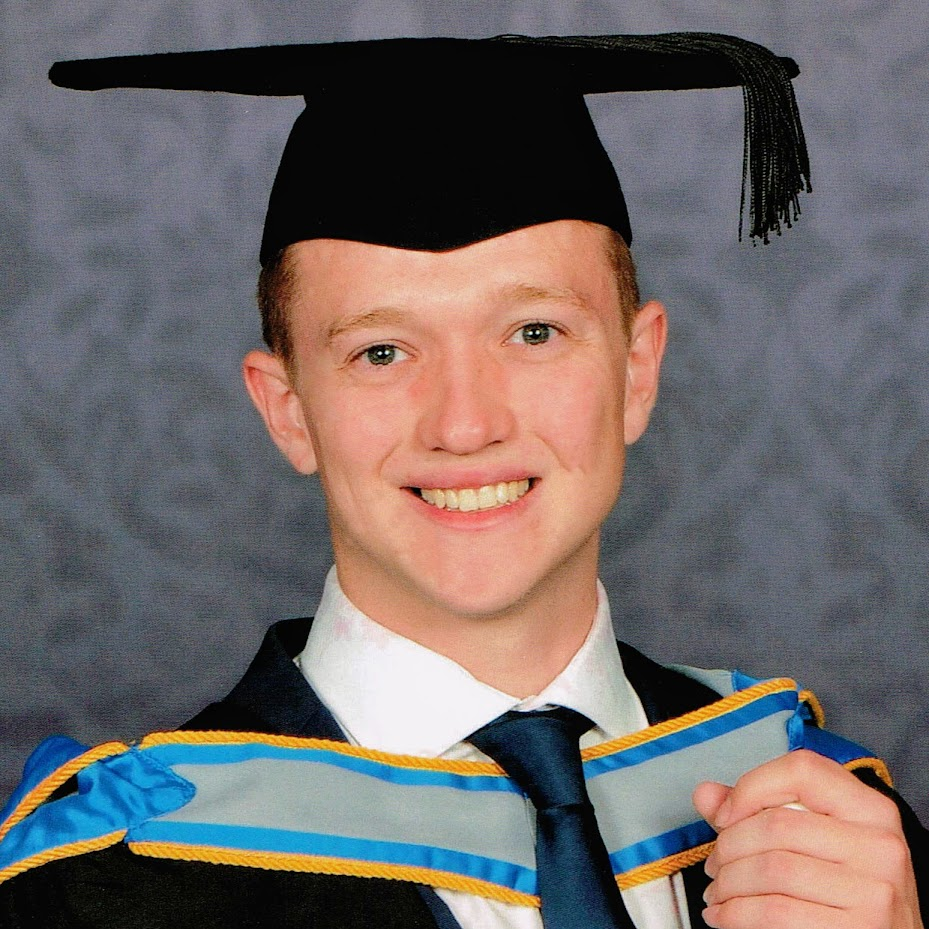
\includegraphics[width=\cvPictureWidth]{Portrait.jpg}
                            };
                        }]
                {};
            \end{tikzpicture}
        \end{center}

        %%%%%%%%%%%%%%%%%%%%%%%%%%%%%%%%%%%%%%%%%%%%%%%%%%%%
        % Profile section
        \ruleline{\textbf{About Me}}
        I am a versatile professional with a strong background in data analysis, software development, and financial management. My recent roles involved developing automation solutions with Python and creating a responsive website using Next.js and React. With a master's degree in mathematics and expertise in MATLAB, R, and Python, I excel at transforming complex data into actionable insights. I am currently seeking software engineering, data science, and data analytics opportunities in Sydney. %

        %%%%%%%%%%%%%%%%%%%%%%%%%%%%%%%%%%%%%%%%%%%%%%%%%%%
        % Contact Section
        \ruleline{\textbf{Contact}}
        \\
        \begin{tikzpicture}[every node/.style={inner sep=0pt, outer sep=0pt}]
            \matrix [
                column 1/.style={anchor=center,contactIcon},
                column 2/.style={anchor=west,align=left,contactIcon},
                column sep=5pt,
                row sep=5pt] (contact) {
                \node{\faMale};
                 & \node{\dob{1996}{01}{15}};            \\
                \node{\faEnvelope};
                 & \node{\href{mailto:leeluderman@googlemail.com}{leeluderman@googlemail.com}};            \\
                \node{\faPhone};
                 & \node{+61 420254547};                    \\
                \node{\faMapMarker};
                 & \node{Sydney \\ NSW 2218, Australia};    \\
                \node{\faLinkedin};
                 & \node{\href{https://www.linkedin.com/in/leeluderman/}{leeluderman}};           \\
                \node{\faGithub};
                 & \node{\href{https://github.com/leele2}{leele2}};           \\
                \node{\faCar};
                 & \node{Car Available, Driving License C}; \\
            };
        \end{tikzpicture}

        %%%%%%%%%%%%%%%%%%%%%%%%%%%%%%%%%%%%%%%%%%%%%%%%%%%
        \ruleline{\textbf{Programming Languages}}
        \skills{{\flag{C.png} C\slash C++/2},{\faCss3 CSS/3},{\faHtml5 HTML/3},{\faReact React/3},{\faGit* Git/4},{\flag{R.png} R/5},{\flag{MatlabLogo.png}\textsc{Matlab}/5.5},{\faPython Python/5.5}}

        \skills

        %%%%%%%%%%%%%%%%%%%%%%%%%%%%%%%%%%%%%%%%%%%%%%%%%%%%%

    \end{minipage}} %
\hfill
%%%%%%%%%%%%%%%%%%%%%%%%%%%%%%%%%%%%%%%%%%%%%%%%%%%%%%%%%
%%%%% MAIN SECTION %%%%%%%%%%%%%%%%%%%%
\adjustbox{valign=t}{\begin{minipage}{11.3cm}
        \vspace*{1cm}
        \section*{{\faGraduationCap} EDUCATION}

        \MySection{2017-2023}{ExeterLogo.png}{Master of Mathematics (MMath)}{University of Exeter}{Exeter, UK}{Upper Second Class (2:1) with Honours}
        {My master’s studies focused on the intersection of mathematics and computer science.\\
            \textbf{Mathematical Modeling with MATLAB:}
            \begin{itemize}
                \item Applied mathematical concepts to real-world problems using MATLAB.
                \item Developed skills in numerical analysis, optimization, and simulation.
            \end{itemize}
            \textbf{Data Analysis and Statistical Modeling with R and Python:}
            \begin{itemize}
                \item Utilized RStudio for data manipulation, visualization, and statistical inference.
                \item Analyzed complex datasets to derive actionable insights.
            \end{itemize}}

        \sectionspace

        %%%%%%%%%%%%%%%%%%%%%%%%%%%%%%%%%%%%%%%%%%%%%%%%%%%
        % Work Experience
        \section*{{\faSuitcase} WORK EXPERIENCE}

        \MySectionB{2022-2023}{RYSA.png}{Restoration Technician}{RYSA Group LTD}{Wagga Wagga, NSW}
        {{Responsibilities \& Achievements}
            \begin{itemize}
                \item Managed data recording and authored comprehensive restoration reports.
                \item Automated customer data processing by developing an email pipeline using Python and the Gmail API.
                \item Designed and launched the company website using the Next.js React framework.
            \end{itemize}}

        \sectionspace

        \MySectionNoPic{2013-2020}{Bookkeeper}{London, UK}{East London Pallets LTD}{{Responsibilities \& Achievements}
            \begin{itemize}
                \item Digitized financial accounts, improving accuracy and efficiency in tracking expenses, sales, and stock.
                \item Implemented a marginal tax scheme, reducing VAT costs through optimized stock records.
                \item Created performance dashboards, providing directors with clear, actionable insights.
                \item Successfully led a change of use application, securing local council approval for the company’s strategic growth.
                \item Developed time-series graphs in R to illustrate the impact of COVID restrictions on business performance, securing government support.
            \end{itemize}}

        %%%%%%%%%%%%%%%%%%%%%%%%%%%%%%%%%%%%%%%%%%%%%%%%%%%
        % Publications
        \section*{{\faBookmark} PROJECTS}

        \publication{Master Thesis}{2022}{Pricing Asian Options in Matlab}{Implemented a well-known pricing model in \textsc{Matlab} and improved its efficiency by reducing the time complexity of the algorithm.}{https://github.com/leele2/Mathematics-in-Business-Project/blob/master/report.pdf}{View on Github}

        \sectionspace

        \publication{End-of-year Project}{2020}{Marine Heat Waves and Their Effects on Phytoplankton}{Analyzed large satellite datasets to identify marine heat waves and model their impact on phytoplankton in R.}{https://github.com/leele2/Research-in-Mathematical-Sciences---CA3/blob/main/report.pdf}{View on Github}

        \sectionspace

    \end{minipage}} %

%%%%%%%%%%%%%%%%%%%%%%%%%%%%%%%%%%%%%%%%%%%%%%%%%%%%%%%%%%%%
% Second Page
\newpage

\sidebar{sideBarColor!25}
\newpageheader{titleBackColor}{Lee}{Luderman}{}{white}

% %%%%%%%%%%%%%%%%%%%%%%%%%%%%%%%%%% SIDEBAR %%%%%%%%%%%%%%%%%%%
\adjustbox{valign=t}{%
    \begin{minipage}{7.3cm}
        \vspace*{0.4cm} % text starts 0.4cm under the top the header

        %%%%%%%%%%%%%%%%%%%%%%%%%%%%%%%%%%%%%%%%%%%%%%%%%%%%
        % Skill and Strengths 
        \ruleline{\textbf{Soft Skills and Strengths}}
        \vspace*{-0.5cm}
        \begin{center}
            \cvtag{Effective Communication}\cvtag{Problem Solving}\cvtag{Team Collaboration}\cvtag{Leadership}\cvtag{Adaptability}\cvtag{Time Management}\cvtag{Attention to Detail}\cvtag{Critical Thinking}\cvtag{Conflict Resolution}\cvtag{Decision-Making}\cvtag{Emotional Intelligence}\cvtag{Client Relations}\cvtag{Flexibility}\cvtag{Interpersonal Skills}\cvtag{Resilience}
        \end{center}

        %%%%%%%%%%%%%%%%%%%%%%%%%%%%%%%%%%%%%%%%%%%%%%%%%%%%
        % Professional Skills 
        \ruleline{\textbf{Professional Skills}}
        \begin{center}
            \cvtag{Data Analysis}\cvtag{Data Visualization}\cvtag{Statistical Modeling}\cvtag{Project Management}\cvtag{Client Relations}
        \end{center}

        %%%%%%%%%%%%%%%%%%%%%%%%%%%%%%%%%%%%%%%%%%%%%%%%%%%
        % Other Interests
        \ruleline{\textbf{Other Interests}}
        \small
        \begin{multicols}{2}
            \begin{itemize}
                \item[\flag{gymnastics.png}] Gymnastics
                \item[\faDumbbell] Gym
                \item[\faPlane] Travelling
                \item[\faMotorcycle] Motorbiking
                \item[\faGamepad] Gaming
                \item[\faChessRook] Chess
            \end{itemize}
        \end{multicols}

        %%%%%%%%%%%%%%%%%%%%%%%%%%%%%%%%%%%%%%%%%%%%%%%%%%%%%
        % QR Code
        \ruleline{\textbf{Download My CV}}
        \scriptsize
        \centering
        Get the latest version of my CV via the QR code below.
        \begin{center}
            \quad
            \qrcode[height=2cm]{
                https://github.com/leele2/CV} \\
            \vspace*{0.5cm}
        \end{center}

    \end{minipage}
}%
\hfill
%%%%%%%%%%%%%%%%%%%%%%%%%%%%%%%%%%% MAIN %%%%%%%%%%%%%%%%%%%%%%%%%
\adjustbox{valign=t}{%
    \begin{minipage}{11.3cm}
        \vspace*{0.4cm}
        %%%%%%%%%%%%%%%%%%%%%%%%%%%%%%%%%%%%%%%%%%%%%%%%%%%
        % Technical Expertise and Applications
        \section*{{\faDesktop} Technical Expertise and Applications}

        \ITCcompetence{Data Analysis}
        {
        \textbf{Python}:
        {Analyzed a dataset containing approximately 2 million nested data points related to job listings on Indeed (UK) during the COVID-19 pandemic. Calculated key metrics to assess the broader job market, drawing conclusions about the impact of COVID restrictions and their influence on employment trends.}\\
        \textbf{R}:
        {Investigated the effects of marine heatwaves on phytoplankton using large spatial-temporal datasets recorded by satellites (e.g., sea-surface temperature and chlorophyll concentration). Employed regression analysis and developed an ARIMA model to describe the causal relationship between these variables.}\\
        }

        \sectionspace

        \ITCcompetence{Modeling and Simulation}
        {
        \textbf{\textsc{Matlab}}:
        {Conducted extensive research on option pricing theory for a master's thesis, exploring the binomial option pricing model and the Black-Scholes method. Developed an alternative numerical model for path-dependent (Asian) options, which eliminated the need for path searching, significantly reducing computational complexity while maintaining accuracy. Validated the model through Monte Carlo simulations and corroborated the results with established findings in the literature.}\\
        }

        \sectionspace

        \ITCcompetence{Software Development \& Automation}
        {
        \textbf{Next.js}:
        {Developed a company website using React, Tailwind CSS, and HTML within the Next.js framework. Integrated dynamic features that interact with the company’s reporting software API, displaying real-time data on job completions and geographical coverage.}\\
        \textbf{Automation}:
        {Automated a manual data entry task by developing a Python script utilizing the Gmail API to scan business emails for new work orders. Extracted information from attached PDFs and populated reporting software autonomously. Deployed the script on a headless Raspberry Pi with remote update capabilities via Git.}\\
        }

        \sectionspace

        %%%%%%%%%%%%%%%%%%%%%%%%%%%%%%%%%%%%%%%%%%%%%%%%%%%
        % Certificates
        \section*{{\faCertificate} CERTIFICATES}

        \adjustbox{valign=t}{\begin{minipage}{2cm}
                \begin{center}
                    
\includegraphics[width=1.8cm]{harvard.jpg}
                \end{center}
            \end{minipage}}
        \hfill \vline \hfill
        \adjustbox{valign=t}{\begin{minipage}{9cm}
                \begin{itemize}
                    \scriptsize
                    \item CS50: Introduction to Computer Science (\textit{EDX, 2020})
                    \item CS50's Web Programming with Python and JavaScript (\textit{EDX, 2021})
                \end{itemize}
            \end{minipage}}

        \vspace*{0.2cm}

        %%%%%%%%%%%%%%%%%%%%%%%%%%%%%%%%%%%%%%%%%%%%%%%%%%%
        % Personal Achievements
        \section*{{\faTrophy} Personal Achievements}
        \vspace*{-0.5cm}
        \begin{multicols}{2}
            \raggedcolumns
            \begin{itemize}
                \footnotesize
                \item \textbf{International Competitor}: Represented England at the Cheerleading Worlds competition, placing 5th.
                \item \textbf{National-Level Gymnast}: Secured 2nd place in the UK at a national gymnastics competition, demonstrating exceptional athletic skill and dedication.
                \item \textbf{Olympic Performer}: Performed in halftime entertainment shows for the London 2012 Olympics, showcasing talent on an international stage.
                \item \textbf{Entertainment Experience}: Participated in television, film productions, and live shows, performing for audiences exceeding 20,000 people.
                \item \textbf{First-Generation University Graduate}: Broke new ground as the first in my family to attend university, illustrating resilience and a commitment to academic and personal growth.
            \end{itemize}
        \end{multicols}


    \end{minipage}}

\end{document}
